%for testing sectioning purpose
% \section{Test thu}
% \input{chapters/sections/sections2.1

\section{Microcontroller}
  \subsection{Theory}
  \gls{mcu} is a small size, special purpose computer. It is small enough in order to be integrated on a small circuit in which will do specified tasks or applications. MCU itself comes with memory, input, output peripherals and processor. Program to run the MCU is stored in \gls{rom} and usually not change in production. A microcontroller is usually designed to run in small size and at low cost, which is compatible to be embedded in other system in order to control actions of the system automatically.

  Few advantages of \gls{mcu} over a microprocessor can be listed as following:
  \begin{itemize}
    \item A MCU is already a standalone microcomputer.
    \item Because it can be considered as an independent computer, most needed components are integrated on a small size board.
    \item The above reason leads to the benefit that using MCU can make the system compact, highly mobile and cost efficiency.
    \item Time reduction because it is programed to run specified set of commands only.
    \item It is also easy to use and maintain.
    \item MCU nowadays usually designed to be used with low power in order to last longer under energy-limited condition.
  \end{itemize}

  \subsection{Microcontroller structure}
  Figure~\ref{fig:mcuStructure} demonstrates the basic structure of a microcontroller. It is easily to see the basic design of a microcontroller and its components.
  \begin{figure}[!ht]
    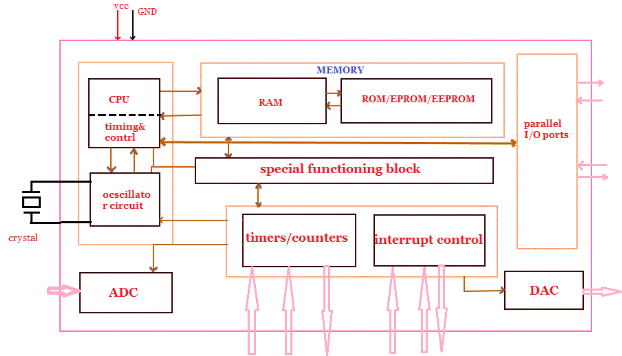
\includegraphics[scale=0.9]{images/Microcontroller-Structure.png}
    \caption{Structure of Microcontroller}
    \label{fig:mcuStructure}
  \end{figure}
  
  \begin{itemize}
    \item CPU: is the central unit which is assembled with \gls{alu} and a \gls{cu}. Its functions are connect parts of the MCU into a single system by doing fetch, decode and execution.
    \item Memory: there are two types of Memory that are required, namely \gls{rom} and \gls{ram}. Each type has its own functions, in which ROM will handle the program and the written instructions and RAM can only store temporary data while the program is executing.
    \item Input/Output: the single board system needs input to execute the program as well as outputs to delivery the information for further handling. The I/O peripherals are the interface of the MCU to communicate with or to control other devices.
    \item Bus: bus is the system of wires that used to connect the \gls{cpu} with other peripherals, which means it plays an important role but rarely discussed.
    \item Timers/Counters: they are built-in components for microcontroller, which is used to count in order to handle external events.
    \item Interrupts: is used to interrupt that can be an external or internal one, which helps to execute an instruction(s) while the main program is executing. 
    \item ADC: \gls{adc}, its name says it all, which is a circuit use to convert analogs signal to digital signals. The reason to use ADC is most sensors available on the market can read only analog signal but CPU of the \gls{mcu} can read digital signal only, so a \gls{adc} is necessary for them to communicate.
    \item DAC: \gls{dac} similar to \gls{adc}, DAC is also a circuit which convert digital signals into analog signals for further processing.
  \end{itemize}


  \subsection{Microcontroller market}
  There exists many microcontrollers on the market which come in various sizes and capacities. The list is only containing very few popular MCU that the author knows of.
  \begin{itemize}
    \item Intel 8051
    \item STMicroelectronics STM8S (8-bit), ST10 (16-bit) and STM32 (32-bit)
    \item Atmel AVR (8-bit), AVR32 (32-bit), and AT91SAM (32-bit)
    \item Freescale ColdFire (32-bit) and S08 (8-bit)
    \item PIC (8-bit PIC16, PIC18, 16-bit dsPIC33 / PIC24)
    \item Renesas Electronics: RL78 16-bit MCU; RX 32-bit MCU; SuperH; V850 32-
    bit MCU; H8; R8C 16-bit MCU
    \item PSoC (Programmable System-on-Chip)
    \item Texas Instruments Microcontrollers MSP430 (16-bit), C2000 (32-bit), and
    Stellaris (32-bit)
  \end{itemize}

\section{Communication}
  \subsection{Introduction}
  Nowadays, there are various communication protocols can be used for the thesis, namely I2C, ISP, RS232, RS-485, Bluetooth or Wi-Fi. Each protocol is designed to be suitable for specified purpose with different advantages or disadvantages, which means a perfect protocol does not exist. When making a decision to choose suitable protocols for the thesis, the trade-off between the stabilization and the speed of the communication protocol has been considered carefully.

  In this thesis, RS-485 is chosen as the main way for components in the system to communicate with each other. RS-485 is defined in 1983 not as a protocol but an electrical interface standard and only specifies the drivers and receivers’ characteristics. It is developed in order to make data rate and transmitting distance are inversely proportional. For instance, the data transmitting speed can reach 10 Mbps within distance of 16 meters or if the distance is extended to 1220 meters, the data rate is lower to 100 kbps. The advantage of RS-485 over RS232, which is developed in 1960, is multiple nodes can be parallel connected to a bus. Additionally, the network can be extended in length and number of nodes easily by using simple connectors. Besides, Wi-Fi, Bluetooth, GSM and MQTT are also implemented in the thesis in order to take the advantages of different communication protocols in different circumstances.

  
  \subsection{RS-485}
  Table~\ref{table:RS-485HighLightSpecs} shows the remarkable specifications of RS-485. With these characteristics, RS-485 was a robust interface standard and was able to meet the requirements in industries, in which implemented applications that need a stable, fast and reliable connection. 
  
  Figure~\ref{fig:fullHalfDuplex} demonstrates two ways to implement the connection with RS-485, which are full-duplex and half-duplex. Full-duplex implementations require four-wire (two signal pairs) instead of two-wire in half-duplex implementations; But despite the downside of two-wire implementation is it is limited to half-duplex and needs attention to turn-around delay, in practical applications, half-duplex is most chosen. The reason is full-duplex solution depends on master-slave model, which means the slaves cannot communicate with each other. In modern designs of transceiver, the allowed number of nodes can connect to the bus is up to hundreds.
    %RS-485 highlight specs table
    \begin{table}[h!]
      \begin{center}
      \begin{tabular}{ |c||c|  }
        \hline
        Name & Detail\\
        \hline
        Differential&   Yes\\
        Number of supported devices&   32 transmitters/32 receivers\\
        Operation mode & Half-duplex\\
        Longest supported distance & at 100kbps: 1200 meters\\
        Highest supported transmitting speed& at 10Mbps: 16 meters\\
        Mark (data = 1) condition& 1.5V to 5V (A negative towards B)\\
        Space (data = 0) condition& 1.5V to 5V (A positive towards B)\\
        Output current capacity& 250mA\\
        Receiver input sensitivity& $\pm$200 mV\\
        Receiver input range& -7V to 12V\\        
        \hline
       \end{tabular}
       \caption{RS-485 Remarkable Specifications}
       \label{table:RS-485HighLightSpecs}
      \end{center}
      \end{table}
    
    %full-duplex, half-duplex implementation figure
    \begin{figure}[!ht]
      \begin{center}
      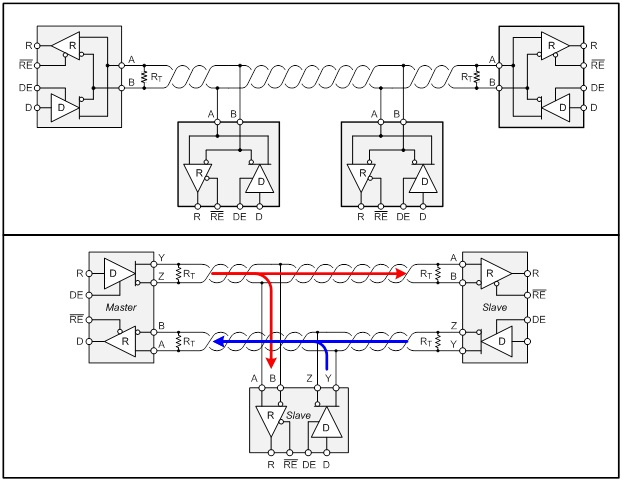
\includegraphics[scale=0.8]{images/rs485-fullduplex-halfduplex.jpg}
      \caption{Half-duplex and Full-duplex implementations}
      \label{fig:fullHalfDuplex}
      \end{center}
    \end{figure}


    Working principle of RS-485 is different in comparison to other standard; Instead of using a zero ground as the voltage reference, which will cause noise over the communication length, it uses floating voltage between two wires of the signal pairs, A and B or (+) and (-). After transmitting, the receiver compares the different of voltage between two wires and achieved the correct data with the lowest noise may cause. Figure~\ref{fig:rs485Wave} illustrates an example of the RS-485 waveforms transmitting one byte which has Mark, Space, and Idle phases. In most network, there will be one node acting as the master and the rest work as the slaves. At this point, the master sends command frame over the connection, and all slaves receive the data, then each slave with different functionality will work as programmed with different received data and also response to the master as programmed. The best practical result is obtained with the use of twisted pair of wires because some of the noise current will flow in the opposite direction with the current in the cable. In case using the straight cable, the noise current flows straightly along the cable in the same direction which will cause a loop current. Combined with the twisted pairs of wires, the cable also comes with shield, which is an accepted approach to restrain the noise, is used in applications that need higher noise resistance.
    \begin{figure}[!ht]
      \begin{center}
        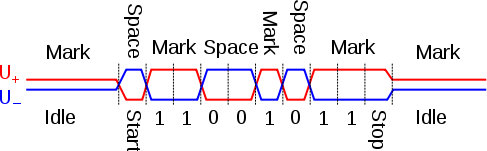
\includegraphics[scale=0.8]{images/RS-485_waveform.png}
        \caption{RS-485 waveform}
        \label{fig:rs485Wave}
      \end{center}
    \end{figure}

    As written in the introduction, RS-485 can connect with multiple transmitters and receivers in the same network. For instance, using input resistance around 12k\si{\ohm},the numbers of devices can connect to the system is up to 32. Besides, with the connecters, this number can increase significantly to the number of thousands and the transmitting distance can be also extended to kilometers. In addition, the network implemented with RS-485 needs termination, usually with a 120\si{\ohm} resistance at the end of two wires. This is applied to terminate or minimize the reflection in order to avoid the fraud of sending data. Furthermore, it usually included pull up and pull down resistors for fail-safe bias in each wire in case that any wire is not controlled by any device. When input voltage ranging from -200mV to +200mV, receiver understands as “undefined” state, which caused by several reasons such as system is shutdown, connection from receiver to network is lost, or cable has an open or short part. In this case, fail-safe biasing is applied in order to confirm that the receivers receive defined states only.

  \subsection{MQTT}
    MQTT is abbreviation of Message Queuing Telemetry Transport, which is a protocol laid in Application layer of OSI model. It is designed as a machine-to-machine and remarkably lightweight protocol that helps communication between constrained devices becomes effortless in comparison to other wireless protocols. In detail, its working principle based on publish and subscribe methodology in order to reduce the amount of transmitting data which leads to the reduction of used bandwidth, latency and power consumption.

    A \gls{mqtt} system is the combination of a server, but usually named broker, and the clients, in which can acts as either a publisher, subscriber or both. One broker can have numerous clients connect to and each client can subscribe to any topic it is programmed. These subscribers are following and watching for the changes of data of the subscribed topics, once other clients which are defined as the publisher publishes message to the topics, then the broker distributed the payload of message to other clients who had subscribed to those topics. In this scenario, the publisher and subscribers do not need to know the information of each other, the only needed are the topics for publishing and subscribing. Figure~\ref{fig:mqttEg} refers a simple example of a MQTT system consists of one broker and four clients, in which three clients are the publishers and one is the subscriber that subscribes to three topics the publishers publish to. To be specific, three publishers are the sensor nodes publish to three topics, temp1, temp2 and temp3; the last client named Sensor Data Gatherer acts as the subscriber that follows three topics mentioned previously. At once, the subscriber will receive the message whenever a publisher broadcasts the message to any of those topics. Implemented MQTT system will be described in details in later part of the thesis.
    \begin{figure}[!ht]
      \begin{center}
        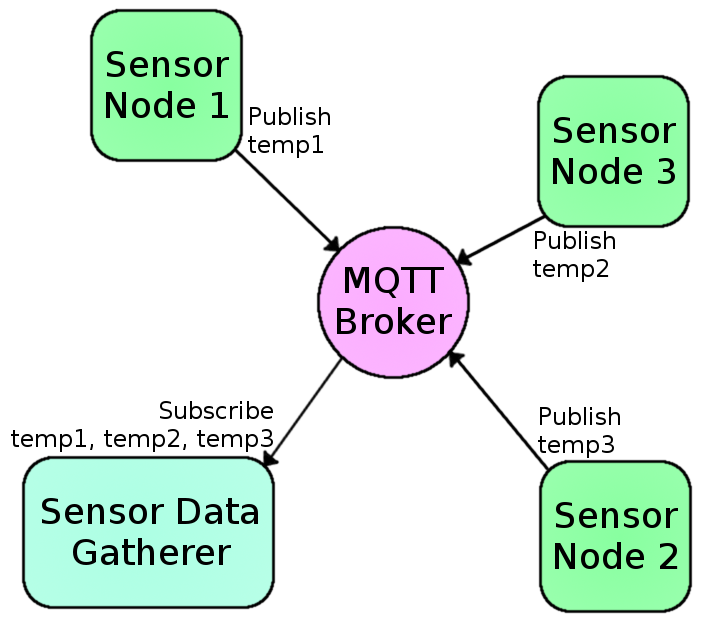
\includegraphics[scale=0.4]{images/mqttEg.png}
        \caption{Simple example of a MQTT system}
        \label{fig:mqttEg}
      \end{center}
    \end{figure}

  \subsection{WebSocket}
    WebSocket was introduced in 2011 in term of a communication protocol, implementing full-duplex channels over one TCP connection. The protocol is laid in Application layer of OSI model but distinguished from HTTP. Distinct to HTTP, in WebSocket applications, a server can send the data to client without waiting for requests from client. All data are being sent between server and client will be sent to a settled connection which helps accelerate the data rate and keep the connection opened when necessary. Similar to \gls{mqtt}, it is designed to reduce the transmitting data, which leads to the reduction of bandwidth and consumed power. Although it is designed for web applications, still, it can be implemented in any applications that need such a lightweight protocol.
    \begin{figure}[!ht]
      \begin{center}
        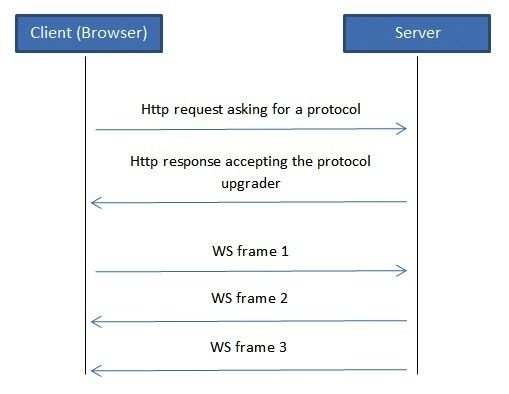
\includegraphics[scale=0.7]{images/ws-1.jpg}
        \caption{WebSocket working principle}
        \label{fig:wsPrinciple}
      \end{center}
    \end{figure}
    Figure~\ref{fig:wsPrinciple} illustrates how WebSocket works. There are two parts of the protocol, handshaking and transmitting data. At first, client sends a request to server to initialize the websocket connection, the server then send an acceptance to connect. After this point, the data are being sent as WS frame with numbering as in the Figure~\ref{fig:wsPrinciple}.

\section{Facial Recognition}
This is a field of Computer Vision, and also considered as a field in Biometrics researches. Facial Recognition is the technique implemented to detect and recognize face(s) in photos or real-time video, then compare to pre-calculated data to predict with probability. In general, face recognition has similar characteristics with fingerprint recognition or iris recognition, the significantly different is the step to extract features of individual field. Iris recognition and fingerprint recognition have plenty of applications with extremely high accuracy, meanwhile face recognition still has difficulties because of its dependent on environment. There are plenty of methodologies to implement a facial recognition, the more difficult and resource cost, the more accurate it is. In this thesis, the author use \gls{lbph}, which is already built in the library named OpenCV.

\gls{lbph} usually comes with two more recognizers, namely EigenFaces Face Recognizer and FisherFaces Recognizer. While Eigenfaces and Fisherfaces are affected significantly by environment light, LBPH is an improvement. The idea is not to find the local features of an image. LBPH algorithm tries to find the local structure of an image, and it does that by comparing each pixel with its neighbouring pixels.
\begin{figure}[!ht]
  \begin{center}
    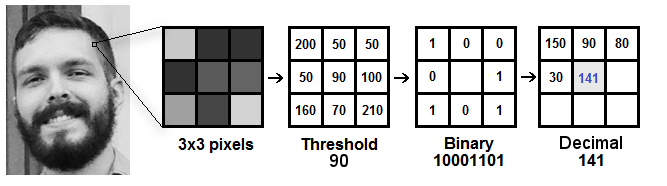
\includegraphics[scale=0.6]{images/lbph.png}
    \caption{How LBPH works}
    \label{fig:lbph1}
  \end{center}
\end{figure}

Based on the Figure~\ref{fig:lbph1}, the process is broke in to smaller steps as following.
\begin{itemize}
\item We have a grayscale face image.
\item Take 3x3 matrix of pixel
\item Present intensity from 0 to 255.
\item Take central value as the threshold and will be use to define new value from the neighbors (this case choose 8).
\item For each neighbor of the central value (threshold), we set a new binary value. We set 1 for values equal or higher than the threshold and 0 for values lower than the threshold.
\item Now, the matrix will contain only binary values (ignoring the central value). We need to concatenate each binary value from each position from the matrix line by line into a new binary value (e.g. 10001101). 
\item Then, we convert this binary value to a decimal value and set it to the central value of the matrix, which is actually a pixel from the original image.
\item At the end of this procedure (LBP procedure), we have a new image which represents better the characteristics of the original image.
\end{itemize}
Now stepping to extract histogram of the above result, please refers to figure~\ref{fig:lbph2}
\begin{figure}[!ht]
  \begin{center}
    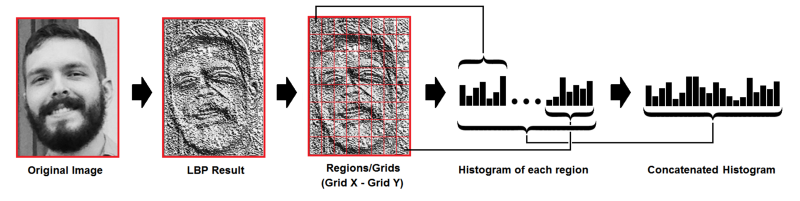
\includegraphics[scale=0.5]{images/lbph2.png}
    \caption{How LBPH works (2)}
    \label{fig:lbph2}
  \end{center}
\end{figure}
\begin{itemize}
\item As we have an image in grayscale, each histogram (from each grid X and Y) will contain only 256 positions (0~255) representing the occurrences of each pixel intensity.
\item Then, we need to concatenate each histogram to create a new and bigger histogram. Supposing we have 8x8 grids, we will have 8x8x256=16.384 positions in the final histogram. The final histogram represents the characteristics of the image original image.
\end{itemize}





  


